\documentclass{ximera}
\title{Images and Graphs}

\begin{document}
\begin{abstract}
    A description of how images and graphs are rendered or included.
\end{abstract}
\maketitle
   
\section*{How Ximera renders Image and Graph Content}

There are several ways to embed graphics into Ximera document. One method is to use \verb|\includegraphics|. Here we see an included a JPEG and a PNG:

\begin{verbatim}
\begin{image}
  %https://commons.wikimedia.org/wiki/File:Lama_LLama_Alpaca_06.jpg
  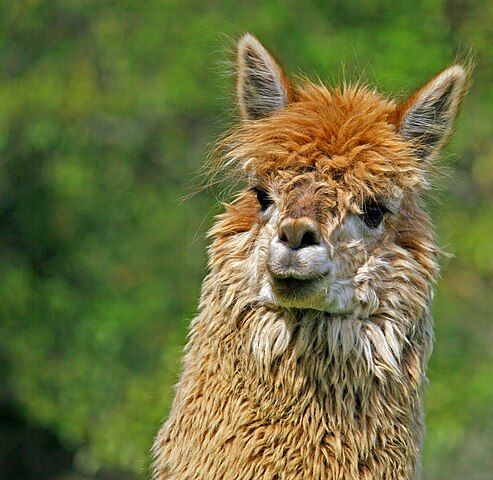
\includegraphics[width=.3\textwidth]{llama.jpg}\qquad
  %https://commons.wikimedia.org/wiki/File:Llama_in_watercolour.png
  
\includegraphics[width=.3\textwidth]{llama.png}
\end{image}
\end{verbatim}
In the code above, the command image is just a Ximera provided wrapper
that can be redefined for printing. It does automatically resize
content though and can be useful for showing images side-by-side:
\begin{image}
  %https://commons.wikimedia.org/wiki/File:Lama_LLama_Alpaca_06.jpg
  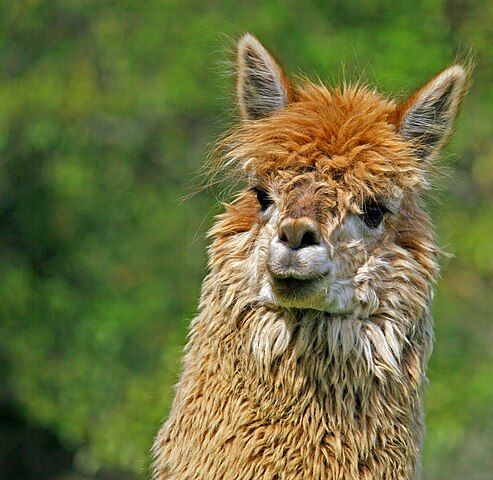
\includegraphics[width=.3\textwidth]{llama.jpg}\qquad
  %https://commons.wikimedia.org/wiki/File:Llama_in_watercolour.png
  
\includegraphics[width=.3\textwidth]{llama.png}
\end{image}

Here we have a pdf
\begin{center}
  
\includegraphics{llama.pdf}
\end{center}


\section{TikZ}
Another way to include graphics is to use Tikz. In some sense this is
preferred, as then the source produces the images.
\begin{image}
  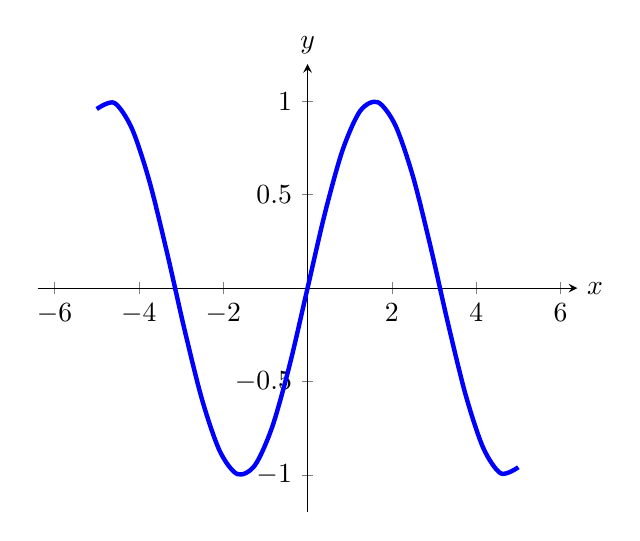
\begin{tikzpicture}
    \begin{axis}[
        xmin=-6.4,
        xmax=6.4,
        ymin=-1.2,
        ymax=1.2,
        axis lines=center,
        xlabel=$x$,
        ylabel=$y$,
        every axis y label/.style={at=(current axis.above origin),anchor=south},
        every axis x label/.style={at=(current axis.right of origin),anchor=west},
      ]
      \addplot [ultra thick, blue, smooth] {sin(deg(x))};
    \end{axis}
  \end{tikzpicture}
\end{image}
\begin{center}
  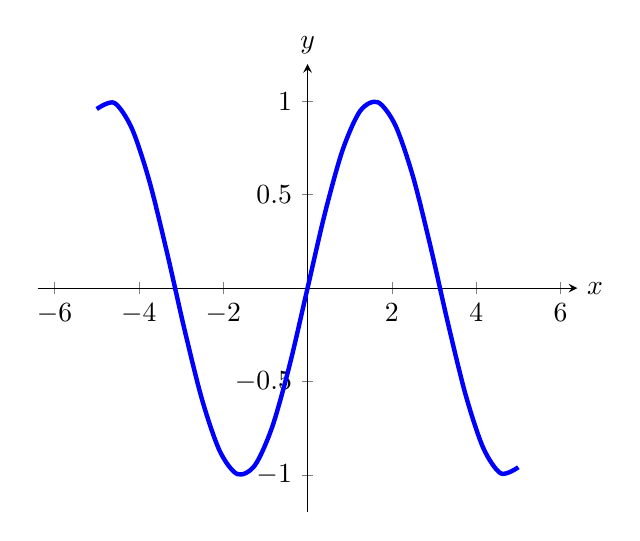
\begin{tikzpicture}
    \begin{axis}[
        xmin=-6.4,
        xmax=6.4,
        ymin=-1.2,
        ymax=1.2,
        axis lines=center,
        xlabel=$x$,
        ylabel=$y$,
        every axis y label/.style={at=(current axis.above origin),anchor=south},
        every axis x label/.style={at=(current axis.right of origin),anchor=west},
      ]
      \addplot [ultra thick, blue, smooth] {sin(deg(x))};
    \end{axis}
  \end{tikzpicture}
\end{center}
\begin{verbatim}
\begin{image}
  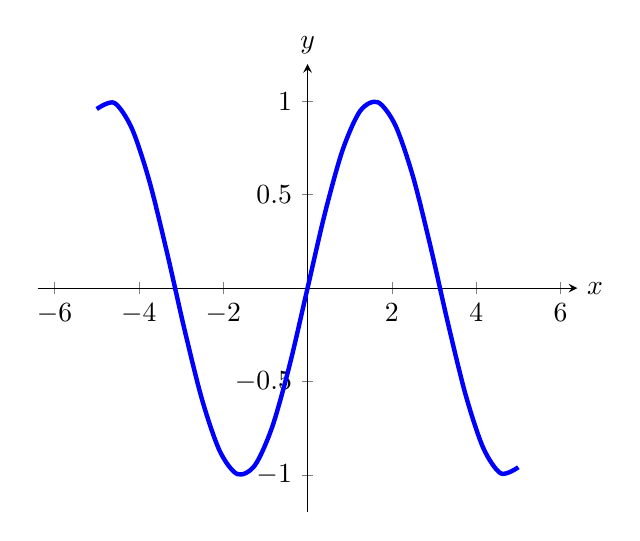
\begin{tikzpicture}
    \begin{axis}[
        xmin=-6.4,
        xmax=6.4,
        ymin=-1.2,
        ymax=1.2,
        axis lines=center,
        xlabel=$x$,
        ylabel=$y$,
        every axis y label/.style={at=(current axis.above origin),anchor=south},
        every axis x label/.style={at=(current axis.right of origin),anchor=west},
      ]
      \addplot [ultra thick, blue, smooth] {sin(deg(x))};
    \end{axis}
  \end{tikzpicture}
\end{image}
\end{verbatim}











\subsection{The graph command}

The easiest way to include an interactive graph is to use the
\verb|\graph| command. Unfortunately, the \verb|\graph| command
doesn't draw a graph in the PDF, rather, it states (in words) that a
graph is produced.
\[
\graph{x^2}
\]
There are a number of options for the \verb|\graph| command:


\paragraph{Change viewing window}

  
\begin{verbatim}
\[
\graph[xmin=-5,xmax=5,ymin=-5,ymax=5]{y=x^2}
\]
\end{verbatim}
\paragraph{Restricting domain}


\begin{verbatim}
\[
\graph{x^2 \left\{ 1 \leq x \leq 10 \right\} }
\]
\end{verbatim}
\paragraph{Default panel displayed}

  
\begin{verbatim}
\[
\graph[panel]{x^2}
\]
\end{verbatim}
\paragraph{Restricting window}

  
\begin{verbatim}
\[
\graph[xmin=0, xmax=10, ymin=0, ymax=10]{x^2}
\]
\end{verbatim}
\paragraph{Axis labels}

  
\begin{verbatim}
\[
\graph[xAxisLabel="time", yAxisLabel="distance"]{y=x}
\]
\end{verbatim}
\paragraph{Hide axes}

  
\begin{verbatim}
\[
\graph[hideXAxis=true, hideYAxis=true]{x^2}
\]
\end{verbatim}
\paragraph{Hide tick marks}

  
\begin{verbatim}
\[
\graph[hideXAxisNumbers=true, hideYAxisNumbers=true]{x=y^2}
\]
\end{verbatim}
\paragraph{Polar graphing}

  
\begin{verbatim}
\[
\graph{r=\theta}
\]
\end{verbatim}
\paragraph{Polar gridlines}


\begin{verbatim}
\[
\graph[polar]{y=x^2}
\]
\end{verbatim}
\paragraph{Graphing a piecewise function}


\begin{verbatim}
\[
\graph{ \sin(x)\left\{x<0\right\}, 2x\left\{ x>=0 \right\} }
\]
\end{verbatim}


\subsection{Desmos}

If you require further features from
\link[Desmos]{https://www.desmos.com/}, you can sign up for an account
and include your worksheets like this:

\begin{verbatim}
\begin{center}
\desmos{zwywds7med}{800}{600}
\end{center}
\end{verbatim}
\begin{center}
\desmos{zwywds7med}{800}{600}
\end{center}



    \subsection*{Any Necessary Content}
    
    
    
    \subsection*{Quirks of Rendering}
    
    
    
    \subsection*{Any Ximera-Specific Optional Arguments}
    
    
    
    \subsection*{Accessibility}
    
    
    
    \subsection*{Potential Problems and Pitfalls}
    
    
    
    \subsection*{Any Best Practices or Advice}
    
    

    
\end{document}
